
\section{Solr}

Begonnen wird der genaue Vergleich mit Solr von Apache.

\subsection{Installation}

Als Systemvoraussetzungen ist eine Java Version $> 8$ gegeben. Es wurde sich hierbei für OpenJDK 11 entschieden. Um Solr im Entwicklermodus auszuführen, kann das entpackte Programm einfach gestartet werden. 
Nach dem ersten Starten wurden 2 Warnungen gemeldet, dass die User-Limits für Solr zu gering sind \ref{lst:warningSolr}. Nachdem diese entsprechend erhöht wurden, verschwanden die Warnungen.

\begin{lstlisting}[language=bash, frame=single, label={lst:warningSolr}] 
  *** [WARN] *** Your open file limit is currently 1024.
  It should be set to 65000 to avoid operational disruption.

  *** [WARN] ***  Your Max Processes Limit is currently 63918.
  It should be set to 65000 to avoid operational disruption.
\end{lstlisting}

Bei der richtigen Installation installiert sich Solr als Service und legt einen eignen Nutzer an. Ein entsprechendes Installations-Skript findet sich dafür im entpackten Solr-Ordner. Sobald dieses mit Root-Rechten aufgerufen wird installiert sich Solr automatisch in das Opt-Verzeichnis.

\subsection{Indexierung}

Um mit der Indexierung starten zu können, muss zuerst ein sogenannter Core erstellt werden. Dieser ist ein Index mit dazugehörigen Transaktions-Log und den Konfigurationsdateien. Nur mit diesen ist es möglich Dateien zu indexieren und auf ihnen zu suchen. Nach der Erstellung lässt sich der Core über die Oberfläche einsehen und zum Teil konfigurieren.

Damit Solr nun die Daten von der Datenbank liest, muss ein DataImportHandler (DIH) \ref{lst:dih} geschrieben werden. In diesen werden die Daten, welche indexiert werden sollen, mit MySQL-Queries eingelesen. Das System setzt dabei auf eine XML-Struktur mit sogenannten Entitys. Diese besitzen jeweils mehrere Attribute, wie den Namen, welcher auf der Oberfläche zur Indexierung angezeigt wird, den MySQL-Query mit dem die Daten gelesen werden und einen Delta-Query, welcher dazu dient, nur die Einträge zu laden, welche Änderungen seit dem letzten Import erlebt haben. 

Der Delta-Query benötigt hierbei eine eigene Zeitstempel-Spalte in der Datenbank, welche angezeigt, wann die Spalte das letzte Mal editiert wurde. Da die Tabellen im Projekt aktuell keine solche Spalte besitzen, kann die Funktion nicht getestet werden.

Innerhalb des Entity-Elements gibt es entweder weitere Entitys, dazu gleich mehr, oder Field-Elemente. Diese besitzen ein Attribut, welches die Spalte der Tabelle ausweist und einen Namen, der das zugehörige Solr-Schema-Element ausweist. 

Entitys können unbegrenzt ineinander verschachtelt werden. Damit Änderungen an einer verschachtelten Entity nach oben richtig weitergegeben werden, gibt es Parent-Delta-Querys. Diese geben die betroffenen Werte an die übergeordnete Entity weiter. Dafür führt der Parent-Delta-Query einen Aufruf an die überliegende Entity-Tabelle aus, in der er mithilfe der Fremdschlüssel-IDs in den betroffen Zeilen herausfindet.

Der DataImportHandler muss, bevor er benutzt werden kann, jedoch noch mit dem Core verbunden werden. Dafür wird dieser, zusammen mit einem JDBC-Treiber in die solrconfig.xml eingetragen. Als JDBC-Treiber wurde in diesem Beispiel der Treiber von MariaDB verwendet.

\begin{lstlisting}[language=xml, frame=single, label={lst:dih}, 
    morekeywords={entity,query,deltaQuery,parentDeltaQuery,field,column, name}] 
    <entity name="lemma" 
      query="select * from lemma" 
      deltaQuery="select eid from lemma 
        where last_modified > '${dataimporter.last_index_time}'"> 
		<field column="bezeichnung" name="bezeichnung" />
    [...]
    <entity name="lemma_gnd" 
      query="select * from lemma_gnd where fk_lemma='${lemma.id}'"
      deltaQuery="select * from lemma_gnd 
        where last_modified > '${dataimporter.last_index_time}'"
      parentDeltaQuery="select * from lemma 
        where id=${lemma_gnd.fk_lemma}">
			
        <entity name="gnd" 
          query="select * from gnd where id = '${lemma_gnd.fk_gnd}'"
          deltaQuery="select * from gnd 
            where last_modified > '${dataimporter.last_index_time}'"
          parentDeltaQuery="select * from lemma_gnd where fk_gnd=${gnd.id}">
          <field column="nummer" name="gnd_nummer" />
          <field column="schlagwort" name="gnd_schlagword" />
          [...]
        </entity>
      </entity>  
    </entity>
\end{lstlisting}

Wie schon eben angesprochen, muss das Solr-Schema für die entsprechende Elemente auch angepasst werden. Dieses Schema dient dazu die Dateitypen für eine möglichst gute Indexierung auszuweisen. Dafür wird zuerst der Dateityp für die Tabellen-Spalte angegeben. Hierbei werden bei den Grundtypen, zum Beispiel unter anderem String und Text\_de gelistet. Dabei wurde angenommen, dass die beiden nur bei Abfragen von unterschiedliche Sprachen einen Unterschied besitzen. Dies ist allerdings falsch. Als eine Abfrage gestellt wurde, die alle Lemmata mit den Buchstaben S finden sollten, kamen mehr Ergebnisse als erwartet zurück. Dies liegt daran, dass Text\_de, das Feld aus Volltext ausweist. 
Bei Volltexten wird jedes Wort einzeln betrachet und so kamen Lemma, in welchen eines der Wörter mit S begann in die Auflistung. Deswegen wurde daraufhin das Feld als String deklariert, was es ermöglicht hat nur Ergebnisse herauszufiltern, welche mit S beginnen.

Es gibt mehrere Möglichkeiten diese Einträge auszuweisen. In diesem Ersteindruck wurden die Einträge über die Administrations-Oberfläche angelegt. Es ist allerdings auch möglich eine eigene Schema-Datei zu erstellen. Diese Methode soll allerdings nicht mehr verwendet werden, da es die Möglichkeit gibt, die Einträge per API zu generieren. Dadurch wird direkt überprüft, ob die Einträge formal stimmen. So können keine fehlerhaften Schemata gebaut werden. Die Einträge, welcher über die API oder die Administrations-Oberfläche gestellt werden, werden in einer Datei namens managed\_schema \ref{lst:managedSchema} im XML-Format angelegt.


\begin{lstlisting}[language=xml, frame=single, label={lst:managedSchema}, 
    morekeywords={type,uninvertible,indexed,stored,field,multiValued, name}] 

    [...]
    <field name="ddc_webdewey_is_checked" type="boolean" 
        uninvertible="false" indexed="true" stored="true"/>
    <field name="description" type="text_de" uninvertible="false" 
        multiValued="true" indexed="true" stored="true"/>
    <field name="erweiterung" type="text_de" 
        uninvertible="false" indexed="true" stored="true"/>
    [...]

\end{lstlisting}

Die Indexierung lief eine Minute und 34 Sekunden für rund 14 Tausend Einträge \ref{img:solrIndexTime}. Dabei wurde der gegebene Arbeitsspeicher nicht komplett ausgenutzt, was darauf schließen lässt, dass die Datenbank der limitierende Faktor war. Die hohe Anzahl der Abfragen ist darauf zurückzuführen, dass Solr keine Joins verwendet, sondern bei jeder verschachtelten Entity die gesamten Tabellen wieder und wieder nach passenden Einträgen durchsucht.

\begin{figure}
	\centering
	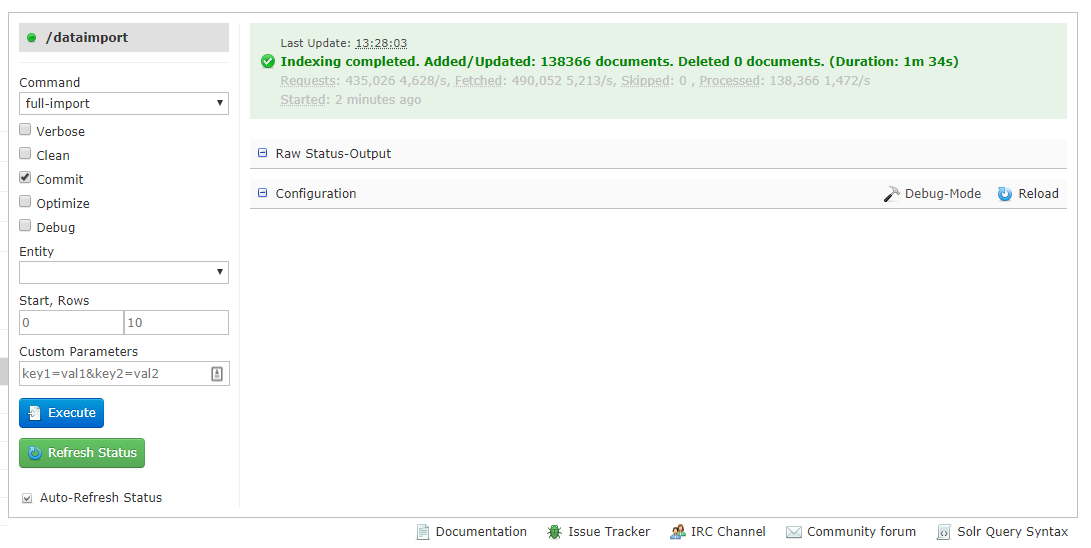
\includegraphics[width=1\linewidth]{images/solr_indexing_time.png}
	\caption{Oberfläche der Indexierung mit Laufzeit.}
	\label{img:solrIndexTime}
\end{figure}

\subsection{Oberfläche}

Die Startseite des Solr-Systems bietet direkten Einblick in auf die Auslastung des Systems \ref{img:solrInterface}. Der Fehler-Log ist auch sehr einfach mit einem Klick zu erreichen. Um an die Statistiken des aktuellen Cores zu kommen, kann dieser aus einen Drop-Down-Menu ausgewählt werden. Positiv anzumerken ist, dass es möglich ist Schema Einträge direkt in der Weboberfläche zu löschen und anzulegen. Es ist jedoch nicht möglich, den DataImportHandler direkt zu verändern, ohne weitere Einstellungen im System vorzunehmen. Es gibt eine Möglichkeit Abfragen direkt über den Web-Oberfläche zu senden, was das Testen der Abfragen erleichtert. Auch bei der Indexierung kann ein Debug-Modus dazu geschaltet werden \ref{img:solrIndexTime}. Zudem besteht die Möglichkeit die Konfigurationsdateien des Cores auf der Weboberfläche einzusehen. Die Dateien dort direkt zu editieren, ist jedoch nicht möglich.
Es gibt keine Möglichkeit Updates direkt über die Weboberfläche einzuspielen. Auch ist diese Seite nicht Responsive geschrieben. 
\begin{figure}
	\centering
	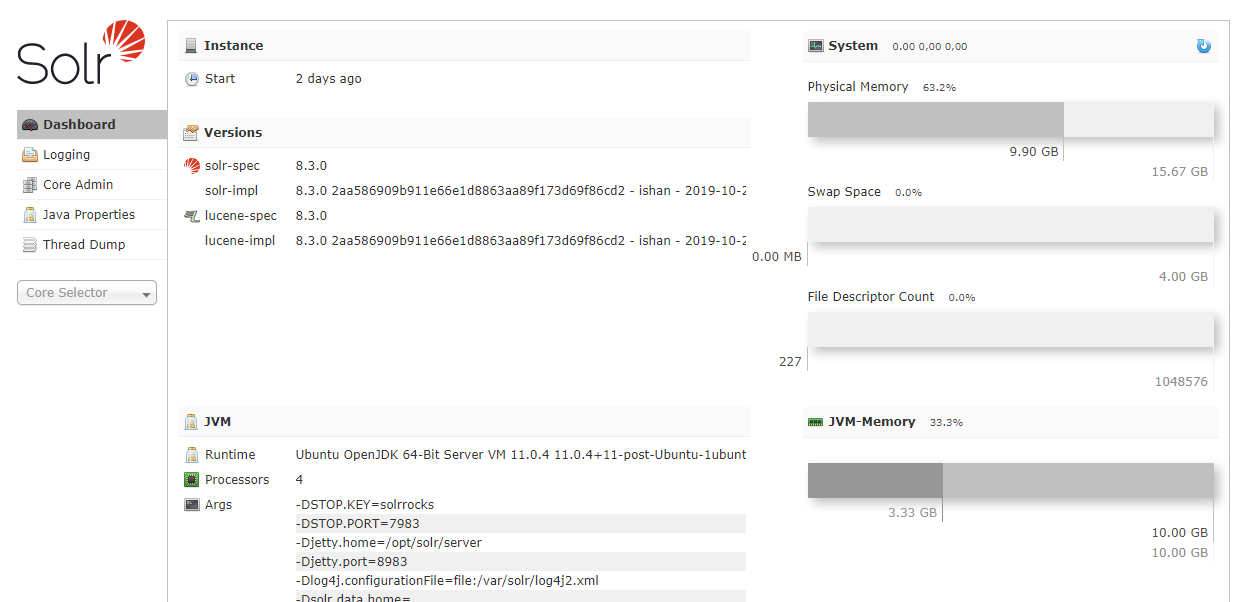
\includegraphics[width=1\linewidth]{images/solr_interface.png}
	\caption{Startseite der Weboberfläche von Solr.}
	\label{img:solrInterface}
\end{figure}


\subsection{Dokumentation}

Die Dokumentation war bei diesem kurzen Test meine Hauptquelle. Die Installation ist dort genau beschrieben. Positiv aufgefallen ist dabei die genaue Beschreibung der Systemvoraussetzungen. Das Team hat mehrere Java-Versionen getestet und alle dort aufgeführt. 
Generell gibt es für alle Themen eine kleine Übersichtsseite, welche die grundlegenden Funktionen erklärt, ohne sich dabei in Details zu verlieren. 
Die Seite für den DataImportHandler hat anhand eines Beispiels gut die Struktur erklärt. Allerdings wäre ein Verweis, dass für die DataImportHandler-Attribute noch extra ein Solr-Schema-Attribut benötigt wird, schön gewesen.
Die Dokumentation ist gut bebildert und bietet einen guten Einstiegspunkt in das System.

\subsection{Absetzen einer Anfrage und Integration in PHP}

Um nicht direkt mit der JSON-API arbeiten zu müssen, gibt es diverse Bibliotheken, die ein wenig der Arbeit abnehmen. Eine der größten ist hierbei Solarium, welches sich mit Composer\footnote{Abhängigkeiten-Manger für PHP} installieren lässt. Da die Composer Technologie schon im Projekt verwendet wird, ist dies vom Vorteil.
Die Query ist herbei sehr einfach, da die Daten beim Import schon dementsprechend indexiert wurden.

\begin{lstlisting}[language=php, frame=single, label={lst:SolrPhp}, 
  morekeywords={type,uninvertible,indexed,stored,field,multiValued, name}] 

  [...] # Imports and variable declarations

  $config = array(
      'endpoint' => array(
          'localhost' => array(
              'host' => '136.199.34.55',
              'port' => 8983,
              'core' => 'dietrich'
  )));
  $queryText = 'original_bezeichnung:S*';
  $solr = new Client($config);
  $query = $solr->createSelect();
  $query->setQuery($queryText);
  $query->setRows(2147483647); 
  [...] # Loop with Timer
  $resultSet = $solr->select($query);
  $count = $resultSet->count();
  [...] # Output Runtime
\end{lstlisting}

Die maximale Anzahl der Zeilen die von Solr geladen werden, sind standardmäßig auf 10 limitiert. Erst mit setRows kann die Anzahl erhöht werden. Für diesen Test wurde der maximale Integer-Wert gewählt, um immer alle Ergebnisse zu bekommen. Damit nun ein guten Median-Wert gebildet werden kann, wurde die Abfrage 100 mal laufen gelassen. Dabei lief die Abfrage durchschnittlich 1.01 Sekunden um die 15838 Ergebnisse herauszusuchen. 
